\documentclass{article}
\usepackage{tikz}

\begin{document}
  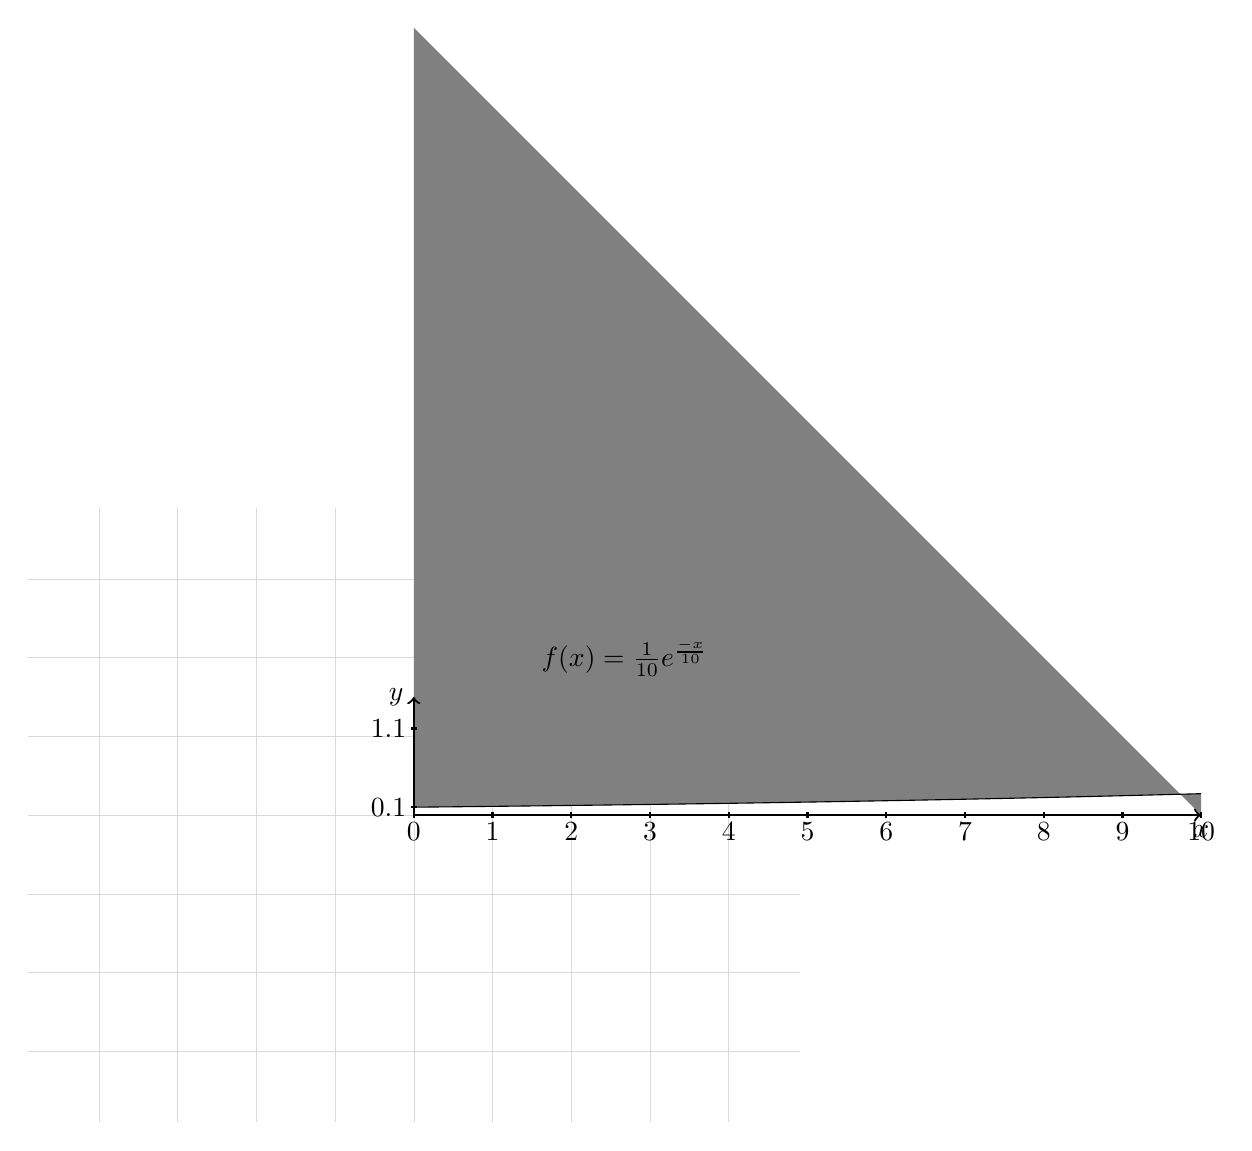
\begin{tikzpicture}
    \draw[very thin, gray!30, step=1 cm](-4.9,-3.9) grid (4.9,3.9);

    \fill [gray, domain=0:10, variable=\x]
      ( 0, 10)
      -- plot ({\x}, {(1/10) * exp(\x/10)})
      -- (10, 0)
      -- cycle;

    \draw [thick] [->] (0,0)--(10,0) node[right, below] {$x$};
     \foreach \x in {0,...,10}
       \draw[xshift=\x cm, thick] (0pt,-1pt)--(0pt,1pt) node[below] {$\x$};

    \draw [thick] [->] (0,0)--(0,1.5) node[above, left] {$y$};
     \foreach \y in {0.1,...,1.5}
       \draw[yshift=\y cm, thick] (-1pt,0pt)--(1pt,0pt) node[left] {$\y$};

    \draw [domain=0:10, variable=\x]
      plot ({\x}, {(1/10) * exp(\x/10)}) node[right] at (1.5,2) {$f(x)=\frac{1}{10}e^{\frac{-x}{10}}$};

  \end{tikzpicture}
\end{document}
